Dans un système ayant deux PONEs et deux TAREs (en plus du revendeur, du marché de gros et de l'AMI), pour être satisfaite rapidement, la demande du client doit se baser sur la sommes des énergies fournies par les 2 PONEs. Par contre, les TAREs ne peuvent acheter qu'à un seul lot d'énergie d'un PONE à la fois (via le marché de gros). C'est donc le revendeur qui doit gérer le rassemblement des 2 retours de TARE pour construire la réponse au client.
\\[1cm]
Ce scénario n'a pas été réalisé dans notre projet par manque de temps car nous devions réaliser des modifications importantes dans notre code et finir le rapport, nous avons pris la décision de ne pas le faire.
Cependant nous avons quand même réfléchi à celui-ci et comment nous l'aurions implémenté si nous avions eu le temps.

\begin{figure}[h]
    \centering
    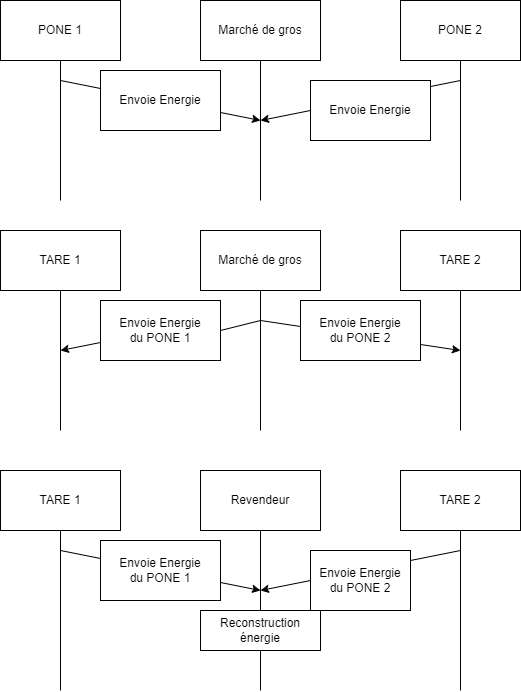
\includegraphics[width=110mm, height=140mm]{images/ScenarioD.png}
    \caption{Schéma du scénario D}
    \label{img:mesh25}
\end{figure}
\newpage